
%%% Local Variables: 
%%% mode: latex
%%% TeX-master: t
%%% End: 
\documentclass[hyperref=true]{beamer}

% Package and Theme
% Some more packages will be used.
\usepackage{amsmath}
\usepackage{amssymb}
\usepackage{algorithmic}
\usetheme{AnnArbor}
\graphicspath{{Figure/}{figures/}{figure/}{pictures/}{picture/}{pic/}{pics/}}


% Make preparation. Make slides. And create wealth by yourself.
% Presentation. Homework. Software Engineering reading.

\begin{document}
\title[Change the World]{How to Change the World with Donald Knuth}
\author{Abraham Xiao}
\institute[Masdar Institute]{Masdar Institute of Science and
  Technology}
\date[CIS612 Presentation]{Information Security Project Presentation}



\begin{frame}
  \titlepage{}
\end{frame}

\begin{frame}
  \tableofcontents{}
\end{frame}

% \begin{column}{width=0.5te}
%   
% \end{column}
% \begin{frame}
%   \begin{columns}
    
%   \end{columns}
% \end{frame}

\section{Discrete Logarithm}
\label{sec:discrete-logarithm}



\begin{frame}
  \frametitle{Discrete Logarithm in a Nutshell}
The security of many cryptographic techniques depends on the
intractability of discrete logarithm problem.\\[4pt]A partial list of these
include:
\begin{itemize}
\item Diffie–Hellman key agreement and its derivatives.
\item ElGamal encryption.
\item ElGamal signature scheme and its variants.
\end{itemize}
General setting for algorithms in this section are:
\begin{itemize}
\item A (multiplicatively written) finite cyclic group $G$
\item $n$ is the order of group $G$
\item $\alpha$ is a generator of group $G$\footnote{For more math
    background, refer to~\cite{Rosen:2012}.}
\end{itemize}
\end{frame}

\begin{frame}
  \frametitle{Relevant Definitions}
Cyclic group and its generator.
  \begin{definition}
    A group is \emph{cyclic} if there is an element $\alpha\in G$ such
    that for each $b\in G$ there is an integer $i$ with
    $b=\alpha^{i}$. Such an element $\alpha$ is called a generator of $G$.
  \end{definition}
Discrete logarithm.
  \begin{definition}
    Let $G$ be a finite cyclic group of order $n$. Let $\alpha$ be a
    generator of $G$, and let $\beta\in G$. The \emph{discrete
      logarithm of $\beta$ to the base $\alpha$}, denoted
    $\log_{\alpha}\beta$, is the unique integer $x$, $0\leq x\leq
    n-1$, such that $\beta=\alpha^{x}$\cite{Menezes:1996:HAC:548089}.
  \end{definition}
\end{frame}


\begin{frame}
  \frametitle{A Discrete Logarithm Example}
  \begin{example}
    Let $p=97$. Then $\mathbb{Z}_{97}^{*}$ is a cyclic group of order
    $n=96$. A generator of $\mathbb{Z}_{97}^{*}$ is $\alpha=5$. Since
    $5^{32}\equiv 35\mod 97$, $\log_{5}35 =32$ in $\mathbb{Z}_{97}^{*}$.
  \end{example}
\end{frame}

% http://v.youku.com/v_show/id_XNjQ0MzYwMDMy.html 
% Add this link to a possible place
\begin{frame}
  \frametitle{The Diffie–Hellman Problem}
The Diffie–Hellman problem is closely related to the well-studied
discrete logarithm problem.
\begin{definition}
  The \emph{Diffie–Hellman problem} is the following: given a prime
  $p$, a generator $\alpha$ of $\mathbb{Z}_{p}^{*}$, and elements
  $\alpha^{a}\mod p$ and $\alpha^{b}\mod p$, find $\alpha^{ab}\mod p$.
\end{definition}
% \\[4pt]
Wait! Could we just possibly do
\begin{equation}
  \label{eq:diffie–hellman-1}
  \alpha^{a}\times\alpha^{b}\rightarrow\alpha^{ab}
\end{equation}
Well, life is not as easy as it looks like\ldots
\begin{equation}
  \label{eq:diffie–hellman-2}
  \alpha^{a}\times\alpha^{b}=\alpha^{a+b}
\end{equation}

\end{frame}

\begin{frame}
  \frametitle{Links between Discrete Logarithm and Diffie–Hellman
    Problem}
\textbf{Suppose} that the discrete logarithm problem in
$\mathbb{Z}_{p}^{*}$ could be efficiently solved\footnote{In math,
  the assumption is as important as,\\ if not more important than
  induction in many situations.}. Then given $\alpha$, $p$,
$\alpha^{a}\mod p$ and $\alpha^{b}\mod p$, one could first find $a$
from $\alpha$, $p$ and $\alpha^{a}\mod p$ by
what?!\\[8pt]\textbf{Solving a discrete logarithm problem}, and  then
compute ${(\alpha^{b})}^{a}=\alpha^{ab}\mod p$.

\end{frame}

\section{ElGamal Cryptosystem}
\label{sec:elgamal-cryptosystem}



\begin{frame}
  \frametitle{ElGamal public-key encryption}
The ElGamal public-key encryption scheme can be viewed as
Diffie--Hellman key agreement\footnote{Yet another fancy nickname for
  key exchange} in key transfer mode.\\
Its security is \textcolor{red}{based on} the intractability of the
discrete logarithm problem (Section~\ref{sec:discrete-logarithm}) and
the Diffie–Hellman problem (Section~\ref{sec:elgamal-cryptosystem}).
\end{frame}


\begin{frame}
  \begin{figure}
    \centering
  \begin{algorithmic}
    \ENSURE~A public key and its corresponding private key is created
    for every entity.
    \STATE~Steps to generate key pairs are described as follows:
    \begin{enumerate}
    \item Generate a prime $p$ that is large enough and cannot be
      predicted, i.e.\ it should be generated randomly. Find a
      generator $\alpha$ of the multiplicative group $\mathbb{Z}_{p}^{*}$ of
      integers modulo $p$.
    \item Randomly select an integer $a$ satisfying $1\leq
      a\leq p-2$. Then calculate $\alpha^{a}\mod p$.
    \item The public key is returned as $(p,\alpha,\alpha^{a})$; The
      private key is returned as $a$.
    \end{enumerate}
  \end{algorithmic}
  \caption{\textbf{Algorithm} Key generation for ElGamal public-key encryption}
  \label{fig:basic-elgamal-encryption}
  \end{figure}
\end{frame}

\begin{frame}
\begin{figure}
  \centering
  \begin{algorithmic}
    \ENSURE~$B$ uses $A$'s public key to encrypt a message $m$. Then
    $A$ uses decrypts using his private key.
    \begin{enumerate}
    \item \emph{Encryption}. The steps for $B$ to take are as follows:
      \begin{enumerate}
      \item Require or obtain $A$'s authentic public key
        $(p,\alpha,\alpha^{a})$. 
      \item Express the plaintext message as an integer in the scale
        ${0,1,\ldots,p-1}$. 
      \item Randomly select an integer $k$ satisfying $1\leq k\leq
        p-2$.
      \item Calculate $\gamma=\alpha^{k}\mod p$ and
        $\delta=m\cdot{(\alpha^{a})}^{k}\mod p$.
      \item Transmit the ciphertext $c=(\gamma,\delta)$ to $A$.
      \end{enumerate}
    \item \emph{Decryption}. The decrypt steps for $A$ are described
      as follows:
      \begin{enumerate}
      \item Calculate $\gamma^{p-1-a}\mod p$ using $A$'s private
        key. (note: due to the characteristic of modulus,
        $\gamma^{p-1-a}=\gamma^{-a}=\alpha^{-ak}$). 
      \item Calculate plaintext $m$ by evaluating
        $(\gamma^{-a}\cdot\delta\mod p)$.
      \end{enumerate}
    \end{enumerate}
  \end{algorithmic}
  \caption{\textbf{Algorithm} ElGamal public-key encryption~\cite{ref:Elgamal1985}}
  \label{fig:basic-elgamal-public-key-encry-algo}
\end{figure}
\end{frame}


% Indian people. Pakistan people. And People's Republic.
\begin{frame}
  \frametitle{ElGamal Encryption with artificially small parameters}
\emph{Key generation}. Entity $A$ selects the prime $p=2357$ and a
generator $\alpha=2$ of $\mathbb{Z}_{2357}^{*}$. $A$ chooses the
private key $a=1751$ and computes
\begin{equation}
  \label{eq:elgamal-encryption-1}
  \alpha^{a}\mod p=2^{1751}\mod 2357=1185
\end{equation}
$A$'s public key is $(p=2357,\alpha=2,\alpha^{a}=1185)$.\\
\emph{Encryption}. To encrypt a message $m=2035$, $B$ selects a random
integer $k=1520$ and computes 
\begin{equation}
  \label{eq:elgamal-encryption-2}
  \gamma=2^{1520}\mod 2537=1430
\end{equation}
and
\begin{equation}
  \label{eq:elgamal-encryption-3}
  \delta=2035\cdot 1185^{1520}\mod 2357=697
\end{equation}
\end{frame}

\begin{frame}
  \frametitle{ElGamal Encryption cont.}
  B sends $\gamma=1430$ and $\delta=697$ to $A$.\\
\emph{Decryption}. To decrypt, $A$ computes
\begin{equation}
  \label{eq:elgamal-encryption-4}
  \gamma^{p-1-a}=1430^{605}\mod 2357=872
\end{equation}
and recovers $m$ by computing 
\begin{equation}
  \label{eq:elgamal-encryption-5}
  m=872\cdot 697\mod 2357=2305
\end{equation}
A clear \textcolor{red}{disadvantage} of ElGamal encryption is that
there is a \emph{message expansion} by a factor of $2$. That is, the
ciphertext is \textcolor{red}{twice} as long as the corresponding
plaintext.
\begin{equation}
  \label{eq:elgamal-encryption-6}
  m=2035\Rightarrow (\gamma=1430,\delta=697)
\end{equation}
\end{frame}




\section{Attack Techniques}
\begin{frame}
  \frametitle{Exhaustive Search}
The most obvious algorithm for discrete logarithm problem is to
successively compute $\alpha^{0}$,$\alpha^{1}$,$\alpha^{2}$,\ldots
until $\beta$ is obtained.\\[8pt]
This method takes $O(n)$ multiplications, where $n$ is the order of
$\alpha$, and is therefore inefficient if $n$ is large (i.e. in cases
of cryptographic interest).\\[8pt]
Say we use $1024$ bits, then the number should be maximum $2^{1024}$
as large.
\end{frame}

\begin{frame}
  \begin{figure}
    \centering
    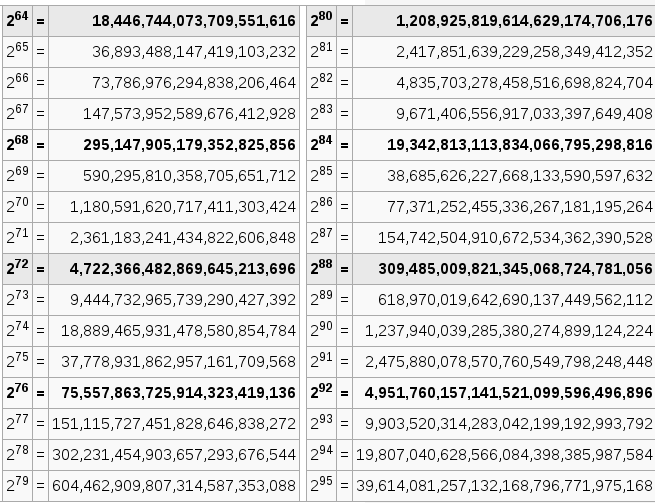
\includegraphics[scale=0.4]{PowOfTwo.png}
    \caption{Power of Two}
    \label{fig:attack-power-of-two}
  \end{figure}
\end{frame}

\begin{frame}
  \frametitle{Index Calculus}
  % Add an example here. Lunch time.
The index-calculus algorithm is the most powerful method known for
computing discrete logarithms. The technique employed
\textcolor{red}{does not} apply to all groups, but when it does (apply
to specific groups), it often gives a subexponential-time algorithm.\\[8pt]
The index-calculus algorithm requires the selection of a relatively
small subset $S$ of elements of $G$, called the \emph{factor base}, in such
a way that a \textcolor{red}{significant fraction} of elements of $G$
can be effectively expressed as \emph{products pf elements} from $S$.
\end{frame}



\begin{frame}[allowframebreaks]
  \frametitle{Index Calculus Toy Example}
Let $p=229$. The element $\alpha=6$ is a generator of
$\mathbb{Z}_{229}^{*}$ of order $n=228$. Consider $\beta=13$. Then
$\log_{6}13$ is computed as follows, using index-calculus technique.
\begin{enumerate}
\item The factor base is chosen to be the first $5$ primes:
  $S={2,3,5,7,11}$.
\item The following six relations involving elements of the factor
  base are obtained (unsuccessful attemps are not shown):
  % \begin{gather}
  %   \label{eq:index-calculus-1}
  %   6^{100}\mod 229=180=2^{2}\
  % \end{gather}
  % \begin{equation}
  %   \label{eq:index-calculus-1}
  %   \begin{split}

  %   \end{split}
  % \end{equation}
% \end{frame}

\begin{center}
$6^{100}\mod 229  = 180 = 2^{2}\cdot 3^{2}\cdot 5$\\
$ 6^{18}\mod 229  = 176 = 2^{4}\cdot 11$\\
$6^{12}\mod 229=176=3\cdot 5\cdot 11$\\
\ldots
\end{center}
\end{enumerate}
\end{frame}


\begin{frame}
These relations yields the following equations involving the
  logarithms of the elements in the factor base:
\begin{center}
$100\equiv 2\log_{6}2+2\log_{6}3+\log_{6}5\mod 228$\\
$18\equiv 4\log_{6}2+2\log_{6}11\mod 228$\\
$12\equiv \log_{6}3+\log_{6}5+\log_{6}11\mod 228$\\
\ldots
\end{center}
% \end{enumerate}
Solving the linear system of six equations in five unknown (the
logarithms $x_{i}=\log_{6}p_{i}$) yields the solutions
$\log_{6}2=21$, $\log_{6}3=208$, $log_{6}5=98$, $\log_{6}7=107$, and
$\log_{6}11=162$. All in modulus.\\[4pt]
Suppose that the integer $k=77$ is selected. Since
$\beta\cdot\alpha^{k}=13\cdot6^{77}\mod 229=147=3\cdot 7^{2}$.
\end{frame}




\section{Appendices}


\begin{frame}[allowframebreaks]
  \frametitle{References}
\bibliographystyle{amsalpha}
\bibliography{Ref}

\end{frame}


\end{document}
